\section{Splinter: Practical, Private Web Application Queries}
\label{chap:splinter}

This chapter presents Splinter, a practical system that protects user
queries to web applications.

\subsection{Motivation}
Many online services let users query large datasets:
some examples include restaurant sites, stock quotes,
medical information, and patents. In these services, 
any user can query the data, and the datasets themselves
are not sensitive. However, web services can infer a great deal of identifiable and sensitive
user information from these queries, such as her 
political affiliation, sexual orientation, income,
medical conditions, behavior, etc.~\cite{narayanan2010myths, narayanan2008robust}.
Web services can use this information maliciously and put users at risk to practices such as
discriminatory pricing~\cite{amazon-disc-pricing, price-disc2, hannak2014measuring}.
For example, online stores have charged users different prices based on location~\cite{price-disc}, and
travel sites have also increased prices for certain frequently searched flights~\cite{travel-pricing}.
Even when the services are honest, server compromise and subpoenas can leak the sensitive user
information on these services~\cite{ravichandran2009capturing, yelp-compromise, twitter-compromise}.

This paper presents Splinter, a system that protects users' queries to web applications
while achieving practical performance for many current web applications.
In Splinter, the user divides each query into shares and sends them to different
\emph{providers}, which are services hosting a copy of the dataset (Figure~\ref{fig:overview}).
As long as any one of the providers is honest and does not
collude with the others, the providers cannot discover sensitive
information in the query.
However, given responses from all the providers, the user
can compute the answer to her query.

\begin{figure}
	\centering
	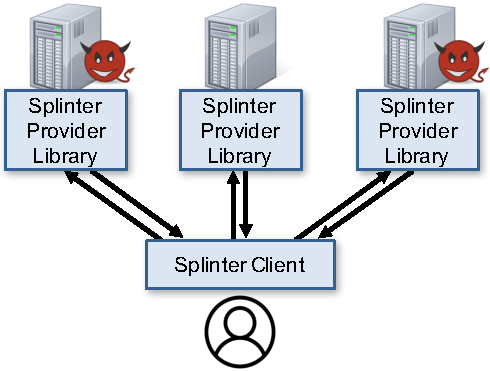
\includegraphics[width=\textwidth]{splinter-figs/overview.pdf}
	\caption[Overview of Splinter architecture.]{
		Splinter architecture. 
		The Splinter client splits each user query into shares and sends them to multiple
		providers. It then combines their results to obtain
		the final answer.
		The user's query remains private as long as any one provider is honest.
	}
	\label{fig:overview}
\end{figure}

Previous private query systems have generally not achieved practical performance
because they use expensive cryptographic primitives and protocols.
For example, systems based on Private Information Retrieval (PIR)~\cite{goldberg,chor1997private,pir-search} require many round trips and high bandwidth for complex queries, while systems based on garbled
circuits~\cite{wu2016,lan2016embark,ben2008fairplaymp} have a high computational cost.
These approaches are especially costly for mobile clients on high-latency networks.

Instead, Splinter is the first system to use and extend a recent cryptographic primitive called
Function Secret Sharing (FSS)~\cite{fss, gilboa2014distributed} for private queries.
FSS allows the client to split certain functions into shares that keep parameters of the
function hidden unless all the providers collude.
With judicious use of FSS, many queries can be answered at low CPU and bandwidth cost in only a single network round trip.

Splinter makes two contributions over previous work on FSS.
First, prior work has only demonstrated efficient FSS protocols for point and interval functions with additive aggregates such as SUMs~\cite{fss}.
We present protocols that support a more complex set of non-additive aggregates such as MAX/MIN and TOPK at low computational and communication cost.
Together, these protocols let Splinter support a subset of SQL that can capture many popular online applications.

Second, we develop an optimized implementation of FSS for modern hardware that leverages AES-NI~\cite{aes-ni} instructions and multicore CPUs.
For example, using the one-way compression functions that utilize modern AES instruction sets, our implementation is 2.5$\times$ faster per core than a na\"ive implementation of FSS.
Together, these optimizations let Splinter query datasets with millions of records at sub-second latency on a single server.

We evaluate Splinter by implementing 
three applications over it: a restaurant review site similar to Yelp, 
airline ticket search, and map routing.
For all of our applications, Splinter can execute queries in less than 1.6 seconds, at a cost of less than 0.02 cents in server resources on Amazon EC2.
Splinter's low cost means that providers could profitably run a Splinter-based service
similar to OpenStreetMap routing~\cite{osm}, an open-source maps service, while only charging users a few dollars per month.

%Finally, Splinter does have some limitations.
%First, FSS, like PIR, requires scanning the whole input dataset on
%every query, to prevent providers from figuring out which records have
%been accessed.
%Second, Splinter does not support some SQL features, such as private join conditions.
%Despite these limitations, we show that Splinter is practical on large
%real-world datasets, such as maps, and can support many of today's online applications.
%Because human-created datasets are unlikely to grow faster than
%hardware capabilities in the future, we believe Splinter's techniques will only
%become more practical over time.

%FSS improves over PIR 
%because it allows matching \textit{multiple} records efficiently in one scan
%while practical PIR schemes can only match a single record in one scan. 
%Therefore, to the best of our knowledge,
%Splinter is the first system to practically preserve the privacy 
%of queries on large public datasets.

In summary, our contributions are:
\begin{itemize}
	\item{Splinter, a private query system that achieves significantly lower CPU and communication costs than previous systems.}
	\item{New protocols that extend FSS to complex queries with non-additive aggregates, e.g., TOPK and MAX.}
	\item{An optimized FSS implementation for modern CPUs.}
	\item{An evaluation of Splinter on realistic applications.}
\end{itemize}

\subsection{Conclusion}
\label{sec:conclusion}
Splinter is a new private query system that protects sensitive parameters
in SQL-like queries while scaling to realistic applications. Splinter uses and extends a recent
cryptography primitive, Function Secret Sharing (FSS),
allowing it to achieve up to an order of magnitude better
performance compared to previous private query systems. We develop
protocols to execute complex queries
with low computation and bandwidth. As a proof of concept,
we have evaluated Splinter with three sample applications---a Yelp clone,
map routing, and flight search---and showed
that Splinter has low response times from 50 ms to 1.6 seconds with low
hosting costs.
